\newpage

\appendix

\section{Dynamic Temporal Sharing}
\label{sec:dts-appendix}

Dynamic Temporal Sharing (DTS) is an adaptive baseline that dynamically adjusts the frequency of switching between inference and finetuning phases based on real-time system conditions. The algorithm (\Cref{alg:dts}) continuously monitors queue lengths, batch sizes, arrival rates, and completion rates to compute a multi-dimensional pressure metric comprising queue pressure ($\text{avg\_queue}/20.0$), spike pressure ($\text{max\_queue}/25.0$), and backlog pressure ($(\text{arrival\_rate} - \text{completion\_rate})/8.0$). Based on the total pressure, DTS adaptively selects finetuning intervals between 64-512 steps using pressure thresholds (pressure $\leq 0.8$ for minimum frequency, pressure $\geq 2.0$ for maximum frequency) and linear interpolation with a $0.6\times$ scaling factor for intermediate values. To ensure system stability, the algorithm incorporates hysteresis through weighted historical averaging ($(\text{frequency} + 2 \times \text{prev\_frequency})/3$), applies stabilization adjustments to computed frequencies, and implements decision delays where frequency recomputation occurs only every third scheduling decision to prevent oscillatory behavior under varying workloads.

\begin{algorithm}[htbp]
\label{alg:dts}
\caption{Dynamic Temporal Sharing}
\begin{algorithmic}[1]
\Require $q$, $b$, $a$, $c$
\State $Q[]$, $B[]$, $r_a$, $r_c$
\State $s$, $f_p$, $d$

\Procedure{Scheduler\_Step}{$q$, $b$, $a$, $c$}
    \State $r_a \leftarrow r_a + a$
    \State $r_c \leftarrow r_c + c$
    \State $Q$.append($q$)
    \State $B$.append($b$)
    
    \State $s \leftarrow s - 1$
    \If{$s \leq 0$}
        \State $d \leftarrow d + 1$
        \If{$d \geq 3$}
            \State $s \leftarrow$ \Call{Compute\_Next\_Interval}{}
            \State $d \leftarrow 0$
        \Else
            \State $s \leftarrow \min(512, f_p \times 1.1)$
        \EndIf
        \State \Call{Reset\_Stats}{}
        \State \Return True \Comment{switch to finetuning}
    \EndIf
    \State \Return False \Comment{continue inference}
\EndProcedure

\Procedure{Compute\_Next\_Interval}{}
    \If{$Q$.empty()}
        \State \Return 64
    \EndIf
    
    \State $\bar{q} \leftarrow$ mean($Q$)
    \State $q_{max} \leftarrow$ max($Q$)
    \State $\bar{b} \leftarrow$ mean($B$)
    \State $\lambda \leftarrow r_a / |Q|$
    \State $\mu \leftarrow r_c / |Q|$
    
    \State $p_q \leftarrow \min(1.0, \bar{q} / 20.0)$
    \State $p_s \leftarrow \min(0.5, q_{max} / 25.0)$
    \State $p_b \leftarrow \max(0.0, (\lambda - \mu) / 8.0)$
    \State $p \leftarrow p_q + p_s + p_b$
    
    \If{$p \leq 0.8$}
        \State $f \leftarrow 64$
    \ElsIf{$p \geq 2.0$}
        \State $f \leftarrow 512$
    \Else
        \State $p_n \leftarrow (p - 0.8) / 1.2$
        \State $f \leftarrow 64 + p_n \times 0.6 \times (512 - 64)$
    \EndIf
    
    \State $f \leftarrow f \times 1.35$ \Comment{stabilization adjustment}
    \State $f_s \leftarrow (f + 2 \times f_p) / 3$
    \State $f_p \leftarrow f_s$
    \State $f_s \leftarrow \max(f_s, 64 + 16)$
    
    \State \Return clamp($f_s$, 64, 512)
\EndProcedure
\end{algorithmic}
\end{algorithm}

\section{Coserving Eviction Rates}
\label{sec:coserving_evictions}
\Cref{tab:coserving_evictions} shows the percentage of inference requests experiencing a KV cache eviction during the evaluation of co-serving under the end-to-end experiment described in \Cref{sec:eval}. Overall, the eviction rates are negliglible. The eviction rate for the Qwen2.5-32B (TP=4) model is 0.29\% for when the inference requests arrive at a rate of 16req/s, and reaches a maximum of 1.20\% when the arrival rate is 20req/s. In all other scenarios, no evictions occurred.

\begin{table}[H]
\centering
\caption{Percentage of requests experiencing an eviction}
\label{tab:coserving_evictions}
\adjustbox{width=\columnwidth,center}{%
\begin{tabular}{|l|c|c|c|c|c|}
\hline
Model & QPS=4 & QPS=8 & QPS=12 & QPS=16 & QPS=20 \\
\hline
Llama-3.1-8B & 0.00\% & 0.00\% & 0.00\% & 0.00\% & 0.00\% \\
Qwen2.5-14B & 0.00\% & 0.00\% & 0.00\% & 0.00\% & 0.00\% \\
Qwen2.5-32B & 0.00\% & 0.00\% & 0.00\% & 0.29\% & 1.20\% \\
\hline
\end{tabular}%
}
\end{table}

\section{Preventing Tenant Interference with Virtual Token Counter}
\label{sec:vtc-integration}

FlexLLM can prevent tenant interference (e.g., noisy neighbor problems) thanks to the Virtual Token Counter (VTC) algorithm~\cite{sheng2024fairness}, which can be combined with our co-serving scheduler. This integration ensures fair resource allocation across tenants while maintaining high GPU utilization.

In multi-tenant PEFT serving, tenants may submit requests at vastly different rates. Without fairness controls, aggressive tenants can monopolize resources and degrade service for others. VTC addresses this by tracking per-tenant service consumption and prioritizing underserved tenants.

Algorithm~\ref{alg:flexllm-vtc} shows the integration of VTC into FlexLLM's token-level scheduling. Key modifications include: (1) per-tenant virtual counters $c_i$ tracking cumulative service, (2) counter lifting when idle tenants rejoin to prevent unfair credit accumulation, (3) fair selection of both inference and finetuning tokens based on minimum counter values, and (4) weighted counter updates reflecting different costs of input ($w_p$), output ($w_q$), and finetuning ($w_r$) tokens.

The integration guarantees bounded fairness across tenants. In the analysis, finetuning requests are treated as a special case of inference requests, allowing us to directly apply results from the Virtual Token Counter analysis~\cite{sheng2024fairness}. Let $W_i(t_1, t_2)$ denote the weighted service received by tenant $i$ and $M$ be the maximum number of tokens. The following lemma and theorems formalize the fairness bounds.

\begin{lemma}
When $Q \neq \emptyset$,
\begin{equation}\label{eq:eq-vtc}
    \max_{i \in Q} c_i - \min_{i \in Q} c_i \le \max(w_p \cdot L_{\text{input}}, \max(w_q, w_r) \cdot M).
\end{equation}
\end{lemma}

\begin{theorem}[Fairness for overloaded tenants]
    For any tenants $f$ and $g$, for any time interval $[t1,t2)$ in which $f$ and $g$ are backlogged, Algorithm~\ref{alg:flexllm-vtc} guarantees
\[
    |W_f(t_1, t_2) - W_g(t_1, t_2)| \leq 2\max(w_p \cdot L_{\text{input}}, \max(w_q, w_r) \cdot M).
\]
\end{theorem}

\begin{theorem}[Fairness for non-overloaded tenants]
    Let $[t_1, t_2)$ be any time interval, $T(t,t2)$ be the total services received for all tenants during $[t,t2)$, $n(t,t2)$ be the number of tenants that have requested services during the interval, and $U$ is the upper bound from Equation~\ref{eq:eq-vtc}.

    Assume a tenant $f$ is not backlogged at $t_1$ and has requested services less than $\frac{T(t,t2)}{n(t,t2)}-5U$ during $[t_1, t_2)$. Then, all of the services requested from $f$ during the interval $[t1,t2)$ will be dispatched.
\end{theorem}

The algorithm remains work-conserving—idle resources are allocated to active tenants—while preventing any single tenant from monopolizing the system. The overhead is minimal: $O(n)$ counters for $n$ tenants, with updates occurring at FlexLLM's existing token-level granularity. This integration preserves FlexLLM's memory optimizations (dependent parallelization, graph pruning) while adding fairness guarantees essential for multi-tenant deployments.

\begin{algorithm}[t]
\caption{FlexLLM with Virtual Token Counter for Fair Co-Serving}
\label{alg:flexllm-vtc}
\begin{algorithmic}[1]
\State \textbf{Input:} Input weight $w_p$, output weight $w_q$, finetuning weight $w_r$, max tokens $M$
\State \textbf{Initialize:} $B \leftarrow \emptyset$, $c_i \leftarrow 0$ for all tenant $i$, $Q \leftarrow \emptyset$
\State
\LeftComment{Monitoring Stream}
\While{True}
    \If{request $r$ from tenant $u$ arrives}
        \If{$\not\exists r' \in Q, tenant(r') = u$}
            \If{$Q = \emptyset$}
                \State $l \gets$ the last tenant left $Q$
                \State $c_u \gets \max\{c_u, c_l\}$
            \Else
                \State $c_u \gets \max\{c_u, \min\{c_i \mid i \in Q\}\}$
            \EndIf
        \EndIf
        \State $Q_u \leftarrow Q_u \cup \{r\}$
    \EndIf
\EndWhile
\State
\LeftComment{Execution Stream}
\While{True}
    \If{can\_add\_new\_requests()}
        \LeftComment{Fair inference selection}
        \While{memory available for inference}
            \State $k \leftarrow \arg\min_{i \in \{tenant(r) \mid r \in Q \text{ is an inference task}\}} c_i$
            \State $r \gets$ the earliest inference request in $Q$ from $k$
            \State Add inference request from $Q_k$ to batch $B$
            \State $c_k \leftarrow c_k + w_p \cdot \text{input\_length}(r)$
        \EndWhile
        
        \LeftComment{Fair finetuning token selection}
        \State $s \leftarrow$ compute\_finetuning\_window()
        \While{$s > 0$ and memory available}
            \State $k \leftarrow \arg\min_{i \in \{tenant(r) \mid r \in Q \text{ is a finetuning task}\}} c_i$
            \State $t \gets \min(s, \text{available})$
            \State Process next $t$ tokens from tenant $k$
            \State $c_k \gets c_k + w_r \cdot t$
            \State $s \leftarrow s - t$
        \EndWhile
    \EndIf
    
    \State Execute decode step for $B$
    \For{each tenant $i$ with tokens generated}
        \State $c_i \leftarrow c_i + w_q \cdot \text{output\_tokens}_i$
    \EndFor
\EndWhile
\end{algorithmic}
\end{algorithm}

\section{Component-wise Memory Breakdown}
\label{sec:memory-breakdown-detailed}

\Cref{fig:memory-breakdown-detailed} shows the component-wise memory breakdown for FlexLLM co-serving LLaMA-3.1-8B with LoRA rank 16. For finetuning memory management, FlexLLM preallocates a fixed budget sufficient for the largest supported PEFT configuration (maximum rank with all target modules enabled). This budget covers PEFT weights, gradients, optimizer momentum values, and low-rank activations. The static allocation strategy prevents memory fragmentation during dynamic co-serving while ensuring deterministic memory bounds regardless of the specific PEFT configurations being served.

\begin{figure}[p]
    \centering
    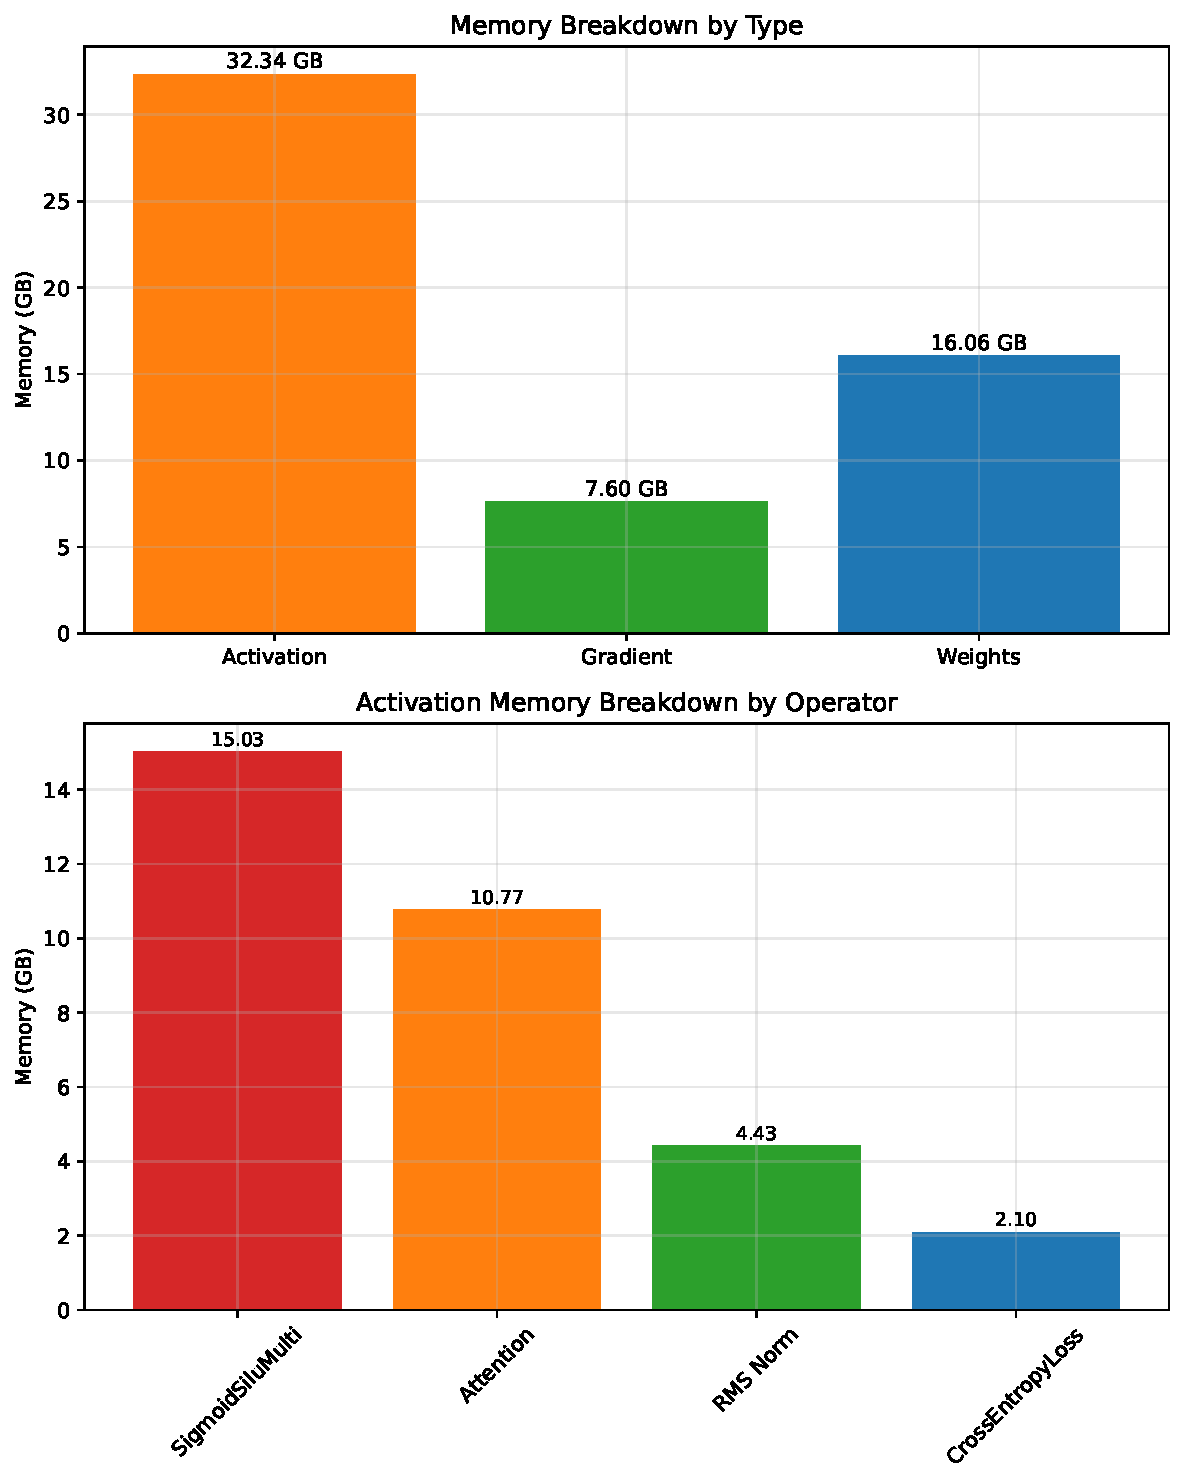
\includegraphics[width=\columnwidth]{utils/memory_breakdown.pdf}
    \caption{Component-wise memory breakdown for FlexLLM co-serving LLaMA-3.1-8B with LoRA finetuning.}
    \label{fig:memory-breakdown-detailed}
\end{figure}

\section{Deployment Considerations}
\label{sec:deployment}

FlexLLM excels in scenarios where its co-serving architecture can maximize resource utilization while maintaining inference performance. \Cref{tab:decision_framework} provides a decision framework to help practitioners identify when FlexLLM delivers optimal benefits.

FlexLLM is particularly well-suited for: (1) inference workloads with moderate burstiness and periods of low utilization, (2) environments with substantial and ongoing finetuning demands, and (3) deployments with moderate SLO requirements (50-100ms TPOT). These conditions allow FlexLLM to fully exploit its co-serving capabilities and memory optimizations.

\begin{table}[t]
\centering
\caption{Decision framework for FlexLLM adoption}
\label{tab:decision_framework}
\adjustbox{width=\columnwidth,center}{%
\small
\begin{tabular}{|l|c|c|}
\hline
\textbf{Scenario} & \textbf{FlexLLM} & \textbf{Separate Clusters} \\
\hline
Bursty inference + high finetuning & \checkmark & \\
Consistent high inference load & & \checkmark \\
Minimal finetuning requirements & & \checkmark \\
Moderate SLOs (50-100ms TPOT) & \checkmark & \\
Strict SLOs (<25ms TPOT) & & \checkmark \\
Cost-sensitive deployments & \checkmark & \\
Operational simplicity priority & & \checkmark \\
\hline
\end{tabular}%
}
\end{table}

FlexLLM's implementation comprises approximately 9K lines of code distributed across compilation, scheduling, memory management, and kernel integration components. The system leverages advanced techniques in GPU programming, distributed systems, and ML compiler optimizations to achieve its performance gains.

Under stricter SLO requirements, FlexLLM's performance characteristics follow predictable queueing theory principles: co-serving introduces service time variance that can affect tail latencies. This trade-off between resource efficiency and latency guarantees becomes more pronounced as SLO targets approach inherent inference latency bounds, making FlexLLM most effective in moderate SLO environments where it can fully utilize its resource optimization capabilities.

\section{Artifact}
The artifact is available at \url{https://github.com/FlexLLM/artifact}. Follow the instructions in the README to build FlexLLM and reproduce the experiments in this paper.